% Source: printed p. 91; PDF p. 100
một độ giãn $E$, rồi trả về lực truyền qua vật liệu $M$ khi nó được kéo đến độ giãn $E$. Đó là một hàm $e:\ulcorner\text{một vật liệu}\urcorner\times\ulcorner\text{một độ giãn}\urcorner\to\ulcorner\text{một lực}\urcorner$. Hàm này nhận đồng thời hai đầu vào, nhưng curry hóa đầu vào thứ hai sẽ thuận tiện. Nhớ rằng $\operatorname{Hom}_{\mathbf{Set}}(\ulcorner\text{một độ giãn}\urcorner,\ulcorner\text{một lực}\urcorner)$ là tập hợp các đường cong lực--độ giãn lý thuyết. Curry hóa biến đổi $e$ thành một hàm
\[e':\ulcorner\text{một vật liệu}\urcorner\to\operatorname{Hom}_{\mathbf{Set}}(\ulcorner\text{một độ giãn}\urcorner,\ulcorner\text{một lực}\urcorner).\]
Đây là một cách thuận tiện hơn để đóng gói cùng lượng thông tin: mỗi vật liệu $M$ có một đường cong lực--độ giãn $e'(M)$. Mệnh đề 3.4.2.3 sẽ diễn đạt điều này chính xác.

\noindent\textbf{Ký hiệu 3.4.2.1.} Cho $A,B$ là các tập hợp. Đôi khi ta ký hiệu tập hợp các hàm từ $A$ đến $B$ là $B^A$,
\begin{equation*}B^A:=\operatorname{Hom}_{\mathbf{Set}}(A,B).\tag{3.21}\end{equation*}

\noindent\textbf{Bài tập 3.4.2.2.} Với một tập hợp hữu hạn $A$, gọi $|A|\in\mathbb N$ là số phần tử của $A$. Nếu $A,B$ đều hữu hạn, kể cả khả năng một hoặc cả hai tập hợp rỗng, có phải luôn đúng rằng $|B^A|=|B|^{|A|}$ không?

\noindent\textbf{Lời giải 3.4.2.2.} Nếu $A,B$ đều rỗng, câu trả lời có thể gây tranh luận; ngoài trường hợp đó, $|B^A|=|B|^{|A|}$ là đúng. Trở lại vấn đề gây tranh luận, một số người nói $0^0$ không xác định, có lẽ vì điều xảy ra với giới hạn trong giải tích: $\lim_{x\to0}x^0=1$, trong khi $\lim_{y\to0}0^y=0$. Nhưng nếu ta xem các số tự nhiên là những lớp đẳng cấu của các tập hợp hữu hạn, thì với $0=|\varnothing|$, chắc chắn cách tốt nhất là xem $0^0=1$, vì $\operatorname{Hom}_{\mathbf{Set}}(\varnothing,\varnothing)=\underline1$. Chọn quy ước $0^0=1$ trong $\mathbb N$, câu trả lời trở thành có, không kèm điều kiện.

\noindent\textbf{Mệnh đề 3.4.2.3 (Curry hóa).} \emph{Cho $A$ là một tập hợp. Với mọi tập hợp $X,Y$, có một song ánh}
\begin{equation*}\phi:\operatorname{Hom}_{\mathbf{Set}}(X\times A,Y)\xrightarrow{\cong}\operatorname{Hom}_{\mathbf{Set}}(X,Y^A).\tag{3.22}\end{equation*}
\begin{proof}[Chứng minh]
Giả sử cho $f:X\times A\to Y$. Định nghĩa $\phi(f):X\to Y^A$ như sau: với mỗi $x\in X$, định nghĩa $\phi(f)(x):A\to Y$ bằng cách đặt $\phi(f)(x)(a):=f(x,a)$ với mỗi $a\in A$.

Bây giờ, ta xây dựng nghịch đảo $\psi:\operatorname{Hom}_{\mathbf{Set}}(X,Y^A)\to\operatorname{Hom}_{\mathbf{Set}}(X\times A,Y)$. Giả sử cho $g:X\to Y^A$. Định nghĩa $\psi(g):X\times A\to Y$ như sau: với mỗi cặp $(x,a)\in X\times A$, đặt $\psi(g)(x,a):=g(x)(a)$.
% Source: printed p. 92; PDF p. 101
Khi đó, với mỗi $f\in\operatorname{Hom}_{\mathbf{Set}}(X\times A,Y)$, ta có $(\psi\circ\phi)(f)(x,a)=\phi(f)(x)(a)=f(x,a)$; với mỗi $g\in\operatorname{Hom}_{\mathbf{Set}}(X,Y^A)$, ta có $(\phi\circ\psi)(g)(x)(a)=\psi(g)(x,a)=g(x)(a)$. Vì thế, $\phi$ là một đẳng cấu như mong muốn.
\end{proof}

\noindent\textbf{Bài tập 3.4.2.4.} Cho $X=\{1,2\}$, $A=\{a,b\}$, $Y=\{x,y\}$.
\begin{enumerate}[label=\alph*.]
\item Viết ba phần tử khác nhau của $L:=\operatorname{Hom}_{\mathbf{Set}}(X\times A,Y)$.
\item Viết mọi phần tử của $M:=\operatorname{Hom}_{\mathbf{Set}}(A,Y)$.
\item Với mỗi phần tử $\ell\in L$ mà bạn chọn trong phần (a), viết hàm tương ứng $\phi(\ell):X\to M$ được bảo đảm bởi Mệnh đề 3.4.2.3.
\end{enumerate}
\noindent\textbf{Lời giải 3.4.2.4.}\keepwithnext
\begin{enumerate}[label=\alph*.]
\item Ta viết từng lựa chọn $\ell_1,\ell_2,\ell_3\in L$ dưới dạng bảng:
\begin{center}\begin{tabular}{c|cc}$\ell_1$&1&2\\\hline$a$&$x$&$x$\\$b$&$x$&$y$\end{tabular}\qquad\begin{tabular}{c|cc}$\ell_2$&1&2\\\hline$a$&$y$&$x$\\$b$&$x$&$y$\end{tabular}\qquad\begin{tabular}{c|cc}$\ell_3$&1&2\\\hline$a$&$y$&$x$\\$b$&$y$&$x$\end{tabular}\end{center}
Chẳng hạn, $\ell_1(1,a)=x$ và $\ell_1(2,b)=y$.
\item Ta viết từng $m_1,m_2,m_3,m_4\in M$ dưới dạng bảng:
\begin{center}\begin{tabular}{c|c}$m_1$&\\\hline$a$&$x$\\$b$&$x$\end{tabular}\qquad\begin{tabular}{c|c}$m_2$&\\\hline$a$&$x$\\$b$&$y$\end{tabular}\qquad\begin{tabular}{c|c}$m_3$&\\\hline$a$&$y$\\$b$&$x$\end{tabular}\qquad\begin{tabular}{c|c}$m_4$&\\\hline$a$&$y$\\$b$&$y$\end{tabular}\end{center}
\item Ta viết từng $\phi(\ell_1),\phi(\ell_2),\phi(\ell_3)$ dưới dạng bảng:
\begin{center}\begin{tabular}{c|cc}&1&2\\\hline$\phi(\ell_1)$&$m_1$&$m_2$\end{tabular}\quad\begin{tabular}{c|cc}&1&2\\\hline$\phi(\ell_2)$&$m_3$&$m_2$\end{tabular}\quad\begin{tabular}{c|cc}&1&2\\\hline$\phi(\ell_3)$&$m_4$&$m_1$\end{tabular}\end{center}
\end{enumerate}

% Source: printed p. 93; PDF p. 102
\noindent\textbf{Bài tập 3.4.2.5.} Cho $A,B$ là các tập hợp. Ta đã định nghĩa $B^A:=\operatorname{Hom}_{\mathbf{Set}}(A,B)$, nên có thể viết hàm đồng nhất là $\mathrm{id}_{B^A}:\operatorname{Hom}_{\mathbf{Set}}(A,B)\to B^A$. Trong Mệnh đề 3.4.2.3, hãy thay $X=\operatorname{Hom}_{\mathbf{Set}}(A,B)$, $Y=B$ và $A=A$. Xét hàm
\[\phi^{-1}:\operatorname{Hom}_{\mathbf{Set}}(\operatorname{Hom}_{\mathbf{Set}}(A,B),B^A)\to\operatorname{Hom}_{\mathbf{Set}}(\operatorname{Hom}_{\mathbf{Set}}(A,B)\times A,B),\]
là nghịch đảo của (3.22). Ta có một phần tử chính tắc $\mathrm{id}_{B^A}$ trong miền xác định của $\phi^{-1}$. Áp dụng hàm $\phi^{-1}$, ta thu được một phần tử
\[\mathrm{ev}=\phi^{-1}(\mathrm{id}_{B^A})\in\operatorname{Hom}_{\mathbf{Set}}(\operatorname{Hom}_{\mathbf{Set}}(A,B)\times A,B);\]
chính nó cũng là một hàm,
\begin{equation*}\mathrm{ev}:\operatorname{Hom}_{\mathbf{Set}}(A,B)\times A\to B.\tag{3.23}\end{equation*}
\begin{enumerate}[label=\alph*.]
\item Mô tả hàm $\mathrm{ev}$ theo cách nó tác động lên các phần tử trong miền xác định.
\item Vì sao người ta có thể muốn ký hiệu hàm này là $\mathrm{ev}$?
\end{enumerate}
\noindent\textbf{Lời giải 3.4.2.5.}\keepwithnext
\begin{enumerate}[label=\alph*.]
\item Một phần tử của $\operatorname{Hom}_{\mathbf{Set}}(A,B)\times A$ là một cặp $(f,a)$, trong đó $f:A\to B$ là một hàm và $a\in A$ là một phần tử. Áp dụng $\mathrm{ev}$ lên $(f,a)$ trả về $f(a)$, một phần tử của $B$ như mong muốn.
\item Vì đó là hai chữ cái đầu của từ \emph{evaluate} (tính giá trị): ta tính giá trị của hàm $f$ tại đầu vào $a$.
\end{enumerate}

Nếu $n\in\mathbb N$ là một số tự nhiên, nhớ rằng theo (2.4), có một tập hợp $\underline n=\{1,2,\ldots,n\}$. Với một tập hợp $A$, ta thường viết tắt
\begin{equation*}A^n:=A^{\underline n}.\tag{3.24}\end{equation*}

\noindent\textbf{Bài tập 3.4.2.6.} Ví dụ 3.1.1.7 nói rằng $\mathbb R^2$ là ký hiệu viết tắt của $\mathbb R\times\mathbb R$, nhưng (3.24) nói rằng $\mathbb R^2$ là ký hiệu viết tắt của $\mathbb R^{\underline2}=\operatorname{Hom}_{\mathbf{Set}}(\underline2,\mathbb R)$. Dùng Bài tập 2.1.2.20, Bài tập 3.1.2.12 và đẳng thức $1+1=2$ để chứng minh chúng đẳng cấu, $\mathbb R^{\underline2}\cong\mathbb R\times\mathbb R$.

(Câu trả lời của Bài tập 2.1.2.20 là $A=\{\ctIIIface\}$, tức $\operatorname{Hom}_{\mathbf{Set}}(\{\ctIIIface\},X)\cong X$ với mọi $X$. Câu trả lời của Bài tập 3.1.2.12 là $\operatorname{Hom}_{\mathbf{Set}}(X\sqcup Y,A)\xrightarrow{\cong}\operatorname{Hom}_{\mathbf{Set}}(X,A)\times\operatorname{Hom}_{\mathbf{Set}}(Y,A)$.)

% Source: printed p. 94; PDF p. 103
\noindent\textbf{Lời giải 3.4.2.6.} Ta có $\{\ctIIIface\}\cong\underline1$, một ký hiệu thuận tiện hơn. Ta có
\[\mathbb R^{\underline2}\cong\mathbb R^{\underline1\sqcup\underline1}\cong\mathbb R^{\underline1}\times\mathbb R^{\underline1}\cong\mathbb R\times\mathbb R.\]
Ba đẳng cấu này thu được lần lượt bằng cách dùng $1+1=2$, Bài tập 3.1.2.12, rồi Bài tập 2.1.2.20.

\subsection{Số học của các tập hợp}
Mệnh đề 3.4.3.1 tóm tắt một số tính chất của tích, đối tích và tập hàm, đặt chúng trong một cách nhìn quen thuộc: số học ở bậc tiểu học. Thật ra, ta có thể xem các số tự nhiên đúng nghĩa là những lớp đẳng cấu của các tập hợp hữu hạn; đó chính là mục đích của chúng khi đếm.

Xét quy trình thông thường để đếm các phần tử của một tập hợp $S$, chẳng hạn các con bò trên một cánh đồng. Ta chỉ vào một phần tử của $S$ đồng thời nói ``một'', chỉ vào một phần tử khác của $S$ đồng thời nói ``hai'', rồi tiếp tục cho đến hết. Khi chỉ vào một con bò và nói một số, bạn đang vẽ một đường tưởng tượng nối số ấy với con bò. Nói cách khác, quy trình này chỉ là tạo một đẳng cấu, tức ánh xạ một-một, giữa $S$ và một tập hợp $\{1,2,3,\ldots,n\}$.

Một lần nữa, các số tự nhiên là những lớp đẳng cấu của các tập hợp hữu hạn. Hành vi của chúng, tức số học của các số tự nhiên, phản ánh hành vi của các tập hợp. Chẳng hạn, việc phép nhân phân phối qua phép cộng là một sự thật về lưới các chấm, như trong Ví dụ 3.1.1.2. Mệnh đề sau trình bày những tính chất số học ấy của các tập hợp.

Trong mệnh đề này, đối tích của hai tập hợp $A,B$ được ký hiệu là $A+B$ thay vì $A\sqcup B$. Đây là một ký hiệu hợp lý nói chung và thường được sử dụng.

\noindent\textbf{Mệnh đề 3.4.3.1.} \emph{Các đẳng cấu sau tồn tại với mọi tập hợp $A,B,C$, ngoại trừ một điểm cần lưu ý; xem Bài tập 3.4.3.2.}
\begin{itemize}
\item $A+\underline0\cong A$;
\item $A+B\cong B+A$;
\item $(A+B)+C\cong A+(B+C)$;
\item $A\times\underline0\cong\underline0$;
\item $A\times\underline1\cong A$;
\item $A\times B\cong B\times A$;
% Source: printed p. 95; PDF p. 104
\item $(A\times B)\times C\cong A\times(B\times C)$;
\item $A\times(B+C)\cong(A\times B)+(A\times C)$;
\item $A^{\underline0}\cong\underline1$;
\item $A^{\underline1}\cong A$;
\item $\underline0^A\cong\underline0$;
\item $\underline1^A\cong\underline1$;
\item $A^{B+C}\cong A^B\times A^C$;
\item $(A^B)^C\cong A^{B\times C}$;
\item $(A\times B)^C\cong A^C\times B^C$.
\end{itemize}

\noindent\textbf{Bài tập 3.4.3.2.} Mọi điều trong Mệnh đề 3.4.3.1 đều đúng, trừ một trường hợp: $\underline0^{\underline0}$. Trong trường hợp này, ta được hai câu trả lời mâu thuẫn, vì với mọi tập hợp $A$, kể cả $A=\varnothing=\underline0$, ta đã khẳng định cả $A^{\underline0}\cong\underline1$ lẫn $\underline0^A\cong\underline0$.

Dựa trên định nghĩa của $\underline0,\underline1$ trong (2.4), và của $A^B$ trong (3.21), câu trả lời đúng cho $\underline0^{\underline0}$ là gì?
\noindent\textbf{Lời giải 3.4.3.2.} $\operatorname{Hom}_{\mathbf{Set}}(\varnothing,\varnothing)$ có một phần tử, nên $\underline0^{\underline0}\cong\underline1$.

\noindent\textbf{Bài tập 3.4.3.3.} Với số tự nhiên, cũng đúng rằng nếu $a,b\in\mathbb N$ và $ab=0$ thì $a=0$ hoặc $b=0$. Phát biểu tương tự có đúng với mọi tập hợp không?
\noindent\textbf{Lời giải 3.4.3.3.} Có; nếu $A,B$ là các tập hợp và $A\times B\cong\varnothing$, thì $A=\varnothing$ hoặc $B=\varnothing$.

Theo một nghĩa nào đó, Mệnh đề 3.4.3.1 nói về các đẳng cấu. Nó cho biết việc hiểu đẳng cấu của các tập hợp hữu hạn quy về việc hiểu các số tự nhiên. Nhưng chú ý rằng trong $\mathbf{Set}$ còn diễn ra nhiều điều hơn các đẳng cấu; đặc biệt, có những hàm không khả nghịch.

% Source: printed p. 96; PDF p. 105
Ở bậc tiểu học, có lẽ bạn chưa từng thấy một biểu thức như
\[\underline5^{\underline3}\times\underline3\longrightarrow\underline5.\]
Tuy vậy, trong Bài tập 3.4.2.5, ta đã tìm được một hàm $\mathrm{ev}:B^A\times A\to B$ tồn tại với mọi tập hợp $A,B$. Hàm $\mathrm{ev}$ không phải một đẳng cấu, nên bằng cách nào đó nó không xuất hiện dưới dạng một phương trình số tự nhiên. Nhưng nó vẫn có ý nghĩa quan trọng.\footnote{Nói gần đúng, sự tồn tại của $\mathrm{ev}:\underline5^{\underline3}\times\underline3\to\underline5$ nói rằng: cho một chấm trong lưới chấm $5\times5\times5$ và một trong ba trục, ta có thể biết tọa độ của chấm ấy trên trục đó.} Nếu chỉ xét các con số, dường như ta được thông báo về một hàm quan trọng $\underline{375}\to\underline5$\ctIIInote{Bản gốc in số $\underline{575}$ trong đoạn này, Bài tập 3.4.3.4 và lời giải. Số phần tử đúng là $|\underline5^{\underline3}\times\underline3|=5^3\cdot3=125\cdot3=375$. Vì vậy, ở cả đoạn và bài tập này, bản dịch dùng $\underline{375}$.}, điều khá kỳ lạ. Vấn đề ở đây chính là vấn đề đã gặp trong Bài tập 2.1.2.19.

\noindent\textbf{Bài tập 3.4.3.4.} Giải thích vì sao có một hàm chính tắc $\underline5^{\underline3}\times\underline3\to\underline5$, nhưng không có một hàm chính tắc $\underline{375}\to\underline5$.
\noindent\textbf{Lời giải 3.4.3.4.} Đây là một phiên bản tinh tế hơn của Bài tập 2.1.2.19: biết rằng tồn tại một đẳng cấu giữa hai tập hợp kém hơn rất nhiều so với việc có một đẳng cấu giữa chúng. Vì vậy, dù đúng rằng $\underline5^{\underline3}\times\underline3$ đẳng cấu với $\underline{375}$, ta không có một đẳng cấu giữa chúng; không có một đẳng cấu chính tắc. Nếu chọn một đẳng cấu tùy ý $f:\underline{375}\xrightarrow{\cong}\underline5^{\underline3}\times\underline3$, nó quả thật hợp thành với hàm tính giá trị để cho một hàm
\[\underline{375}\xrightarrow{f}\underline5^{\underline3}\times\underline3\xrightarrow{\mathrm{ev}}\underline5,\]
nhưng hàm đó sẽ tùy ý giống như lựa chọn đẳng cấu ban đầu.

\noindent\textbf{Khẩu quyết 3.4.3.5.}\keepwithnext
\begin{quote}Đúng là một tập hợp đẳng cấu với bất cứ tập hợp nào khác có cùng số phần tử, nhưng đừng vì vậy mà nghĩ rằng nghiên cứu các tập hợp quy về nghiên cứu các số. Những hàm không phải đẳng cấu không thể được nắm bắt trong khuôn khổ các con số.\end{quote}

\subsection{Đối tượng con và hàm đặc trưng}
\noindent\textbf{Định nghĩa 3.4.4.1.} Với một tập hợp bất kỳ $B$, định nghĩa \emph{tập lũy thừa} (power set) của $B$, ký hiệu $\mathbb P(B)$, là tập hợp các tập con của $B$.

% Source: printed p. 97; PDF p. 106
\noindent\textbf{Bài tập 3.4.4.2.}\keepwithnext
\begin{enumerate}[label=\alph*.]
\item $\mathbb P(\varnothing)$ có bao nhiêu phần tử?
\item $\mathbb P(\{\ctIIIface\})$ có bao nhiêu phần tử?
\item $\mathbb P(\{1,2,3,4,5,6\})$ có bao nhiêu phần tử?
\item Vì sao nó được gọi là ``tập lũy thừa''?
\end{enumerate}
\noindent\textbf{Lời giải 3.4.4.2.}\keepwithnext
\begin{enumerate}[label=\alph*.]
\item $|\mathbb P(\varnothing)|=1$.
\item $|\mathbb P(\{\ctIIIface\})|=2$.
\item $|\mathbb P(\{1,2,3,4,5,6\})|=64$.
\item Với mọi tập hợp hữu hạn $X$, ta thấy $|\mathbb P(X)|=2^{|X|}$, tức 2 lũy thừa $|X|$.
\end{enumerate}

\subsubsection*{3.4.4.3\quad Phức đơn hình}
\noindent\textbf{Định nghĩa 3.4.4.4.} Cho $V$ là một tập hợp và $\mathbb P(V)$ là tập lũy thừa của nó. Vì mỗi phần tử $x\in\mathbb P(V)$ là một tập con $x\subseteq V$\ctIIInote{Bản gốc in $x\subseteq U$. Ở đây dùng $V$, tập nền của $\mathbb P(V)$ vừa được cho.}, ta có thể hiểu biểu thức $x\subseteq x'$ với $x,x'\in\mathbb P(V)$. Một tập con $X\subseteq\mathbb P(V)$ được gọi là \emph{đóng xuống} nếu với mọi $u\in X$ và mọi $u'\subseteq u$, ta có $u'\in X$. Ta nói $X$ \emph{chứa mọi nguyên tử} nếu với mỗi $v\in V$, tập một phần tử $\{v\}$ là một phần tử của $X$.

Một \emph{phức đơn hình} (simplicial complex) là một cặp $(V,X)$, trong đó $V$ là một tập hợp và $X\subseteq\mathbb P(V)$ là một tập con đóng xuống, chứa mọi nguyên tử. Các phần tử của $X$ được gọi là \emph{đơn hình} (simplex). Mọi tập con $u\subseteq V$ có số phần tử $|u|$, nên ta có một hàm $X\to\mathbb N$ gửi mỗi đơn hình đến số phần tử của nó.\ctIIInote{Để hàm $X\to\mathbb N$ này xác định, mọi đơn hình $u\in X$ phải hữu hạn; chẳng hạn, điều đó đúng nếu $V$ hữu hạn. Bản gốc chỉ giả sử “$V$ is a set” và chưa nêu điều kiện hữu hạn này.} Tập hợp các đơn hình có $n+1$ phần tử được ký hiệu là $X_n$, và mỗi phần tử $x\in X_n$ được gọi là một \emph{$n$-đơn hình}.\footnote{Có vẻ khác thường khi tập hợp các tập con có hai phần tử lại được ký hiệu là $X_1$, vân vân. Nhưng đây là quy ước chuẩn, vì phù hợp với khái niệm chiều thông thường: mỗi phần tử của $X_1$ tương ứng với một hình một chiều, và tổng quát hơn, mỗi phần tử của $X_n$ có $n$ chiều.}\ctIIInote{Chú thích 7 của bản gốc in “a two-dimensional shape” cho phần tử của $X_1$. Ở đây dùng “một hình một chiều”, đúng với $1$-đơn hình và quy ước $n$ chiều trong cùng câu.} Vì $X$ chứa mọi nguyên tử, tức các tập con có một phần tử, ta có đẳng cấu $X_0\cong V$ và cũng có thể gọi các 0-đơn hình là \emph{đỉnh}. Đôi khi ta gọi các 1-đơn hình là \emph{cạnh}.\footnote{Tôi viết $X_0\cong V$ thay vì $X_0=V$ vì $X_0$ là tập hợp các tập con một phần tử của $V$. Chẳng hạn, nếu $V=\{a,b,c\}$ thì $X_0=\{\{a\},\{b\},\{c\}\}$. Thật ra, đây chỉ là sự câu nệ.}

Vì $X_0\cong V$, ta có thể ký hiệu một phức đơn hình $(V,X)$ chỉ bằng $X$.

% Source: printed p. 98; PDF p. 107
\noindent\textbf{Ví dụ 3.4.4.5.} Cho $n\in\mathbb N$ là một số tự nhiên và $V=\underline{n+1}$. Định nghĩa \emph{$n$-đơn hình}, ký hiệu $\Delta^n$, là phức đơn hình $\mathbb P(V)\subseteq\mathbb P(V)$, tức toàn bộ tập lũy thừa; nó quả thật đóng xuống và chứa mọi nguyên tử.

Ta có thể vẽ một phức đơn hình $X$ bằng cách trước hết đặt mọi đỉnh lên trang dưới dạng các chấm. Với mỗi $x\in X_1$, ta thấy $x=\{v,v'\}$ gồm hai đỉnh, và vẽ một cạnh nối $v,v'$. Với mỗi $y\in X_2$, ta thấy $y=\{w,w',w''\}$ gồm ba đỉnh, và vẽ một tam giác được tô kín nối chúng. Cả ba cạnh cũng được vẽ, vì đã giả sử $X$ đóng xuống.

Các 0-đơn hình $\Delta^0$, 1-đơn hình $\Delta^1$, 2-đơn hình $\Delta^2$ và 3-đơn hình $\Delta^3$ được vẽ dưới đây:
% Source diagram: Art_P76.jpg, visually inspected.
\begin{center}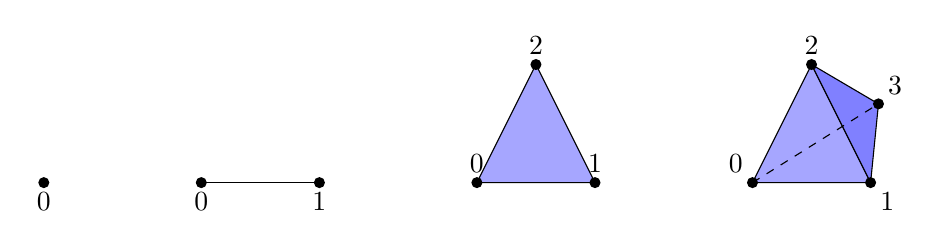
\begin{tikzpicture}[x=1cm,y=1cm]
\fill(0,0)circle(2pt);\node[below]at(0,0){0};
\draw(2,0)--(3.5,0);\foreach\x/\v in{2/0,3.5/1}{\fill(\x,0)circle(2pt);\node[below]at(\x,0){$\v$};}
\filldraw[fill=blue!35](5.5,0)--(7,0)--(6.25,1.5)--cycle;\foreach\x/\y/\v in{5.5/0/0,7/0/1,6.25/1.5/2}{\fill(\x,\y)circle(2pt);\node[above]at(\x,\y){$\v$};}
\filldraw[fill=blue!35](9,0)--(10.5,0)--(9.75,1.5)--cycle;\filldraw[fill=blue!50](9.75,1.5)--(10.6,1)--(10.5,0)--cycle;\draw[dashed](9,0)--(10.6,1);
\foreach\x/\y in{9/0,10.5/0,9.75/1.5,10.6/1}{\fill(\x,\y)circle(2pt);}
\node[above left]at(9,0){$0$};\node[below right]at(10.5,0){$1$};\node[above]at(9.75,1.5){$2$};\node[above right]at(10.6,1){$3$};
\end{tikzpicture}\end{center}
Các $n$-đơn hình với $n\in\mathbb N$ không phải là những phức đơn hình duy nhất. Nói chung, một phức đơn hình là một hợp, hay sự dán ghép các đơn hình theo một cách quy định. Chẳng hạn, xét phức đơn hình $X$ có các đỉnh $X_0=\{1,2,3,4\}$, các cạnh $X_1=\{\{1,2\},\{2,3\},\{2,4\}\}$ và không có đơn hình cao chiều nào, $X_2=X_3=\cdots=\varnothing$. Ta có thể vẽ $X$ như sau:
% Source diagram: Art_P77.jpg, visually inspected.
\begin{center}\begin{tikzpicture}\draw(0,0)--(1.5,0)--(3,0);\draw(1.5,0)--(1.5,-1.5);\foreach\x/\y/\v/\pos in{0/0/1/above,1.5/0/2/above,3/0/3/above,1.5/-1.5/4/below}{\fill(\x,\y)circle(1.8pt);\node[\pos]at(\x,\y){$\v$};}\end{tikzpicture}\end{center}
